\section{Level decomposition and difference budgets}\label{sec:budgets}

We now use $S\to\infty$, as guaranteed by
\Cref{ht:bounded}.  Our inputs are the expanding incidence graph, the
threshold bits $Y_e(v,s)=\mathbf1_{\{n_e(v)>s\}}$, and the coordinate
states $y_x=(A_x,B_{1,x})$ of \Cref{ht:states}.  Recall that an edge is
consistent when precisely its $A$ labels match if its bit is $1$, and
precisely its $B_1$ labels match if its bit is $0$.  The inconsistency
probability $m(v,s)$ satisfies $\int m=O(1)$.
The purpose of this section is to compare two-edge samples at a point or
a center.  Their integrated scores will have a small upper bound from
the product formula and a lower bound recording exceptions to dominant
coordinate labels.  These bounds also hold after conditioning point
stars on a short list of histories.

All level integrals use the weighted measure of \Cref{sec:levels}.
In particular $f=\min(\Prob_E(Y=0),\Prob_E(Y=1))$ and $S=\int f$.
Write $d_{P,\min}=\min_{p\in P}d(p)$ and
$d_{Q,\min}=\min_{q\in Q}d(q)$.

\subsection{Parameters, rare levels, and histories}

The parameters must make prediction errors small even after taking
several samples, while keeping the number of possible histories small
relative to a point degree.

\begin{lemma}[Parameter choice]\label{bud:parameters}
There are integers $K,L,k\to\infty$ such that
\begin{align}
 K\log L&=o(\log t),& D/K&=o(1),\label{bud:KL}\\
 kK\log L&=o(\log t),&
 k^{20}\left((D/K)^{1/4}+L^{-1}+S^{-1}+d_{Q,\min}^{-1}\right)&=o(1).
 \label{bud:hierarchy}
\end{align}
Set $\epsilon=k^{-1/16}$ and
$e_t=(D/K)^{1/4}+L^{-1}$.  Then
$k^3/S=o(1)$, $k^{3+1/16}e_t=o(1)$, and $k=t^{o(1)}$.
\end{lemma}

\begin{proof}
The incidence estimates give $D=o(\log t)$ and $d_{Q,\min}\to\infty$.
For example, first take
$K=\lceil\sqrt{(D+1)\log t}\rceil$ and then choose $L\to\infty$
with $\log L\sim\sqrt{\log t/K}$.  These choices give \eqref{bud:KL}.
Both $K\log L/\log t$ and the parenthesized expression in
\eqref{bud:hierarchy} tend to zero.  Choosing $k\to\infty$ sufficiently
slowly gives \eqref{bud:hierarchy}.  Its stated consequences follow
directly; in particular $k=o(\log t)$ since $K\log L\to\infty$.
\end{proof}

Define the common, damaged, and good rare levels, respectively, by
\[
 \mathcal C=\{f\ge\epsilon\},\qquad
 \mathcal B=\{f<\epsilon,\ m>1/k\},\qquad
 \mathcal G=\{f<\epsilon,\ m\le1/k\}.
\]
Their first two widths satisfy
\begin{equation}\label{bud:widths}
 W_c:=\int\mathbf1_{\mathcal C}\le S/\epsilon,
 \qquad W_b:=\int\mathbf1_{\mathcal B}\le k\int m=O(k)=o(S).
\end{equation}
At each place, $\mathcal C$ is an interval, possibly empty or of zero
length: the function $s\mapsto\Prob_E(n_e(v)>s)$ is nonincreasing.

At a good rare level let $r\in\{0,1\}$ be the minority bit, which is
unique for all sufficiently large $t$.  On every consistent
majority-bit edge the $B_1$ labels match if $r=1$, and the $A$ labels
match if $r=0$.  Thus the mismatch probability of this coordinate is
at most $f+m$.  By \Cref{inc:matching} it has a label $\ell$ whose two
marginal exception probabilities have sum $O(f+m)$.  Fix one such
label measurably, and let $I_x(v,s)$ indicate that the relevant
coordinate of $x$ differs from $\ell$.  Write
\[
 h_P(v,s)=\E_\mu I_p(v,s),\quad
 h_Q(v,s)=\E_\kappa I_q(v,s),\quad
 H_x^*=\int_{\mathcal G} I_x(v,s).
\]
Here and below $I_x$ is used only on $\mathcal G$.  Fixed orderings of
the finite vertex sets settle all choices of labels, so measurability
causes no additional restriction.

\begin{lemma}[Exception mass and joint exceptions]\label{bud:rare-moments}
Uniformly on $\mathcal G$,
\begin{equation}\label{bud:exception-comparison}
 h_P+h_Q\le C(f+m)=o(1),\qquad f\le h_P+h_Q+m.
\end{equation}
Consequently
\begin{equation}\label{bud:first-moments}
 \E_\mu H_p^*+\E_\kappa H_q^*=O(S).
\end{equation}
Furthermore, with $(p,q,r)$ the ordinary wedge law,
\begin{equation}\label{bud:joint-exceptions}
 \int_{\mathcal G}\Prob_E(I_p=I_q=1)=o(S),\qquad
 \int_{\mathcal G}\Prob(I_p=I_r=1)=o(S).
\end{equation}
\end{lemma}

\begin{proof}
The first inequality was just proved, and its right side is uniformly
$O(\epsilon+1/k)=o(1)$.  If both endpoints have the dominant label,
a consistent edge has the majority bit.  Every minority-bit edge
therefore has an exceptional endpoint or is inconsistent, proving the
second inequality.  Integrating and using $\int m=O(1)$ proves
\eqref{bud:first-moments} because $S\to\infty$.

For the joint errors, apply \Cref{inc:rare} with the uniform marginal
bound $a_t=C(\epsilon+k^{-1})\to0$ from
\eqref{bud:exception-comparison}.  Its edge estimate gives
$\Prob_E(I_p=I_q=1)=o(1)(h_P+h_Q)$, and its ordinary-wedge estimate
gives $\Prob(I_p=I_r=1)=o(1)h_P$.  These are exactly the edge and
wedge laws used here.  Both multipliers are uniform over all levels
in $\mathcal G$, so they can be taken outside the integrals.
Equation \eqref{bud:first-moments} then gives
\eqref{bud:joint-exceptions}.
\end{proof}

We next apply the prediction device only to common levels.  When
$W_c>0$, sample a fresh level from their normalized measure and use
\Cref{pred:cross}.  An inconsistent edge accounts for every true
strict-cross failure.  We obtain a fixed history map $H$ with
$|H(P)|\le L^{2K}$ such that, writing $\nu_h$ for the true-state law
of a point of marginal $\mu$ conditional on history $h$ at the fresh
level,
\begin{equation}\label{bud:prediction-error}
 k^3\int_{\mathcal C}\E_E[1-\nu_{H(p)}(R_{y_q})]=o(S).
\end{equation}
Indeed the integral before multiplication by $k^3$ is at most
$\int_{\mathcal C}m+O(W_c e_t)$, and
\Cref{bud:parameters} and \eqref{bud:widths} apply.  If $W_c=0$,
take the empty history, and the assertion is vacuous.

For each center $q$, a \emph{template} is an ordered list
$\theta=(h_1,\ldots,h_k)$ obtained by sampling $k$ independent
neighbors of $q$ and recording their histories.  Let
$a(q,\theta)=\Prob(\theta\mid q)$.  The number $M$ of possible
templates satisfies
\begin{equation}\label{bud:template-count}
 M\le L^{2Kk}=t^{o(1)}.
\end{equation}
The history map is already fixed.  Thus $a(q,\theta)$ uses no fresh
level.  In the joint law
\begin{equation}\label{bud:joint-law}
 \omega(p,q,\theta)=\frac{\mathbf1_{\{(p,q)\in E\}}}{|E|}
                         a(q,\theta),
\end{equation}
the point $p$ and the template are independent conditional on $q$.

\subsection{Three fixed pair experiments}

We use three ways to sample a base and two opposite endpoints:
\begin{enumerate}[label=(\roman*)]
 \item $Q$: sample $q\sim\kappa$, then $p,r$ independently from the
 conditional edge law at $q$;
 \item $P$: sample $p\sim\mu$, then $q,q'$ independently from the
 conditional edge law at $p$;
 \item $P\theta$: sample $(p,\theta)$ from its marginal under
 $\omega$, then $q,q'$ independently from $\omega(q\mid p,\theta)$.
\end{enumerate}
Only positive-mass bases are used.  In each experiment write $x$ for
the base vertex, $y_1,y_2$ for its opposite endpoints, and $Y_1,Y_2$
for the corresponding edge bits.  The base in the third experiment
includes $\theta$.  At a level let
$\rho=\Prob(Y_1=1\mid\text{base})$ under the full indicated law.
These laws are fixed across all levels.  Define
\begin{equation}\label{bud:variations}
 C_i=\int_{\mathcal C}\E_{\mathrm{base}}[2\rho(1-\rho)],
 \qquad i\in\{Q,P,P\theta\}.
\end{equation}

\begin{lemma}[Marginals and diagonal pairs]\label{bud:pair-laws}
Each edge slot of each experiment, after averaging its base, has the
original uniform law on $E$.  For every $p\in P$, the conditional
probability of $q=q'$ in the $P\theta$ experiment, averaged over
$\theta$ conditional on $p$, is at most $M/d(p)$.
\end{lemma}

\begin{proof}
The first assertion is immediate for ordinary stars.  For the third,
the $(p,q)$ marginal of \eqref{bud:joint-law} is the edge law since
$\sum_\theta a(q,\theta)=1$; sampling a conditional slot preserves
this marginal.  More explicitly, a slice of positive probability
$w_\theta=\sum_{p,q}\omega(p,q,\theta)$ has one-edge law
$\omega(p,q,\theta)/w_\theta$ and must be averaged with weight
$w_\theta$.  One can also attach a template independently at a
$Q$ base: conditional on $(q,\theta)$ its two point neighbors still
have their original law, and its single-slot law in each slice is
the same as for $P\theta$.

Fix $p$ and put $a_p(\theta)=\Prob(\theta\mid p)$.  For
$a_p(\theta)>0$,
\[
 \omega(q\mid p,\theta)
 =\frac{\mathbf1_{\{(p,q)\in E\}}a(q,\theta)}{d(p)a_p(\theta)}
 \le\frac1{d(p)a_p(\theta)}.
\]
Its collision probability is at most its largest atom.  Multiplying
by $a_p(\theta)$ and summing over at most $M$ positive-mass templates
gives the asserted bound pointwise in $p$.
\end{proof}

We now define scores that reward matching opposite endpoints and
charge differing bits.  If $Y_1=Y_2=1$, let $N$ be the event that the
$B_1$ labels of $y_1,y_2$ match; if $Y_1=Y_2=0$, let $N$ instead
mean that their $A$ labels match; set $N$ to be false when the bits
differ.  Thus $N$ concerns the coordinate
which a consistent edge of that bit does not share with its base.
For independent bits with parameter $\rho$, equality has probability
$\rho^2+(1-\rho)^2$, whereas disagreement has probability
$2\rho(1-\rho)$. The former is larger except at $\rho=1/2$.
Thus, when equal bits force $N$, a reward slightly above one near
balance and slightly below one elsewhere can give a positive expected
score. The decrease away from balance also makes room for the
increase in the integrated upper bound below.
\Cref{sec:common} will identify the configurations in which equal bits
force the required match.
Set
\[
 \delta=\frac1{100},\qquad \lambda=\frac{\delta^2}{2},\qquad
 c(\rho)=
 \begin{cases}
 1+\lambda,&|\rho-\tfrac12|\le\delta,\\
 1-\lambda,&|\rho-\tfrac12|>\delta.
 \end{cases}
\]
The scalar $\lambda$ is a score coefficient; it is unrelated to the
edge ratios $\lambda_{pr}$ introduced later.
At a good rare level write $r$ for the minority bit. The score is
\[
 \text{score}=
 \begin{cases}
 2I_x\mathbf1_{\{Y_1=Y_2=r,\,N\}},&\text{at a good rare level},\\
 c(\rho)\mathbf1_{\{Y_1=Y_2,\,N\}},&\text{at a common level},\\
 0,&\text{at a damaged level}
 \end{cases}
 -\mathbf1_{\{Y_1\ne Y_2\}}.
\]
Let $D_i$ be the expectation of this score integrated over all
levels in experiment $i$.

The next estimate is the placewise mechanism behind the score
bound.  It identifies exactly when the coefficient $1+\lambda$
can spend more than the available interval length.

\begin{lemma}[Two intervals and a central window]\label{bud:intervals}
Let $b\le b'$, $T\ge0$, and $J$ be an interval of finite length,
with any choice of included endpoints.  Put
$I_-=[b-T,b]$, $I_+=[b',b'+T]$, and
$a=|J\cap I_-|+|J\cap I_+|$, where $|\cdot|$ denotes length.
For $0<\lambda<1$,
\begin{equation}\label{bud:central-envelope}
 \big[(1-\lambda)2T+2\lambda a-2T\big]_+
 \le\lambda|J|\,
       \mathbf1_{\{b,b'\in\operatorname{int}J\}}.
\end{equation}
If $X$ has any probability law on $\R$, and
$|\Prob(X>s)-1/2|\le\delta$ throughout $J$, then
\begin{equation}\label{bud:interior-mass}
 \Prob(X\in\operatorname{int}J)\le2\delta.
\end{equation}
\end{lemma}

\begin{proof}
The left side of \eqref{bud:central-envelope} is $[2\lambda(a-T)]_+$.
For it to be positive both intersections must have positive length,
since either has length at most $T$.  As $J$ is an interval, this
puts both $b,b'$ in its open interior, also when $b=b'$.
Moreover $a\le2T$ and $a\le|J|$, since $I_-$ and $I_+$ have disjoint
interiors.  Hence $2(a-T)\le a\le|J|$.
For \eqref{bud:interior-mass}, take $u<v$ in the interior.  Then
\[
 \Prob(u<X\le v)=\Prob(X>u)-\Prob(X>v)\le2\delta.
\]
Exhausting the open interior by such intervals proves the claim.
The empty-interior case is immediate.  This proof makes no
assumption about atoms at either endpoint of $J$.
\end{proof}

\Cref{fig:budget-intervals} illustrates why positive excess in
\Cref{bud:intervals} requires both thresholds to lie inside the central
window.

\begin{figure}[htbp]
 \centering
 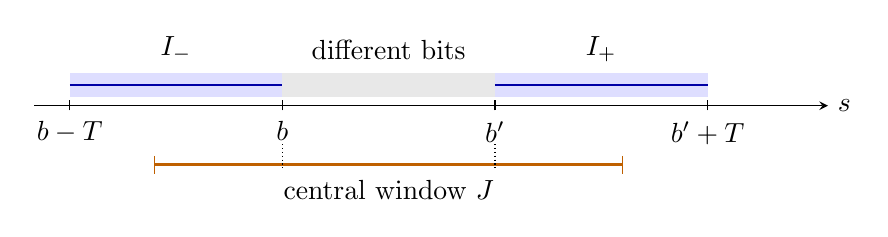
\begin{tikzpicture}[x=0.9cm,y=0.75cm,>=stealth]
 \draw[->] (-0.5,0)--(10.7,0) node[right] {$s$};
 \fill[blue!13] (0,0.15) rectangle (3,0.55);
 \fill[black!9] (3,0.15) rectangle (6,0.55);
 \fill[blue!13] (6,0.15) rectangle (9,0.55);
 \draw[blue!65!black,thick] (0,0.35)--(3,0.35);
 \draw[blue!65!black,thick] (6,0.35)--(9,0.35);
 \node at (1.5,0.95) {$I_-$};
 \node at (4.5,0.95) {different bits};
 \node at (7.5,0.95) {$I_+$};
 \foreach \x/\lab in {0/{b-T},3/{b},6/{b'},9/{b'+T}} {
  \draw (\x,-0.08)--(\x,0.1);
  \node[below] at (\x,-0.1) {$\lab$};
 }
 \draw[orange!75!black,very thick] (1.2,-1.0)--(7.8,-1.0);
 \draw[orange!75!black] (1.2,-0.85)--(1.2,-1.15);
 \draw[orange!75!black] (7.8,-0.85)--(7.8,-1.15);
 \node[below] at (4.5,-1.1) {central window $J$};
 \draw[densely dotted] (3,-0.65)--(3,-1.05);
 \draw[densely dotted] (6,-0.65)--(6,-1.05);
\end{tikzpicture}

 \caption{The intervals $I_-=[b-T,b]$ and $I_+=[b',b'+T]$, with
 $b\le b'$ and $T\ge0$, flank the bit-difference interval.
 The central window $J$ in \Cref{bud:intervals} creates excess only
 if its total overlap with the two flanks exceeds $T$; then both
 thresholds lie strictly inside $J$.}
 \label{fig:budget-intervals}
\end{figure}

\begin{proposition}[Upper score budget]\label{bud:upper}
For each $i\in\{Q,P,P\theta\}$,
\begin{equation}\label{bud:upper-equation}
 D_i\le o(S)+10\delta^2\lambda C_i.
\end{equation}
\end{proposition}

\begin{proof}
First fix a base and two distinct opposite endpoints, and write
$d,d'$ for their incident jumps.  Distinct real endpoints have
distinct $z$ coordinates, so $d\ne d'$.  At a place $v$ let
\[
 b=\min(n_e(v),n_{e'}(v)),\quad b'=\max(n_e(v),n_{e'}(v)),\quad
 u=-\log|d-d'|_v,\quad \alpha=u-b.
\]
The two opposite-endpoint coordinate differences are $d-d'$ and
$1/d-1/d'$ up to signs.  Therefore
\begin{equation}\label{bud:place-identity}
 -\log|(d-d')(1/d-1/d')|_v=2\alpha-(b'-b).
\end{equation}
All thresholds lie within the chosen level interval, so the
integrated bit-difference charge at this place is exactly $b'-b$.

Let $c_v=\log2$ at archimedean entries and $c_v=0$ otherwise.
The triangle inequality gives $\alpha\ge-c_v$, hence
$T_v:=\alpha+c_v\ge0$.  Equality of a grid label at infinity bounds
the corresponding difference by $\sqrt2$ times the grid scale;
at a finite place a matching label bounds it by the scale itself.
If both bits are $1$, a positive charge requires $s<b$ and a
$B_1$ match, which gives
\[
 s\ge b'-\alpha-c_v\ge b-T_v.
\]
If both bits are $0$, the analogous $A$ match gives
$s\ge b'$ and $s\le b+\alpha+c_v\le b'+T_v$.
Thus all positive charges lie in
\begin{equation}\label{bud:positive-intervals}
 I_-=[b-T_v,b],\qquad I_+=[b',b'+T_v].
\end{equation}
Enlarging to these full intervals is legitimate even if part of
them lies outside the chosen level interval.

Suppose a rare positive is counted with minority bit $1$ at a
threshold $s_0$.  Then $s_0<b$ and
$\Prob_E(n_e(v)>s_0)<\epsilon$.  By monotonicity every common level
and every level with minority bit $0$ lies below $s_0$; none can
produce a positive charge in $I_+$.  All minority-$1$ positive
charges lie in $I_-$ by definition.  The case of a rare positive
with minority bit $0$ is symmetric.  Thus, if any rare positive is
counted, all positive charges are on one side, their coefficients
are at most $2$, and their total is at most $2T_v$.

Otherwise only common positives remain.  For this fixed base put
\[
 J_v=\{s:(v,s)\in\mathcal C,\ |\rho(v,s)-1/2|\le\delta\}.
\]
This is an interval because the conditional edge law is fixed
across levels and both restrictions are intervals.  Extend the
coefficient $1-\lambda$ across both full intervals in
\eqref{bud:positive-intervals}, increasing it by $2\lambda$ on
$J_v$.  \Cref{bud:intervals} bounds the excess over $2T_v$ by
\[
 \lambda|J_v|\,
 \mathbf1_{\{n_e(v),n_{e'}(v)\in\operatorname{int}J_v\}}.
\]
This expression is also a valid excess bound in the rare-positive
case, when no excess is needed.  Combining it with the negative
charge and \eqref{bud:place-identity}, then summing over places,
cancels the logarithm by the product formula for the fixed nonzero
element $(d-d')(1/d-1/d')$.  The additive allowance is
$2\sum_v^*c_v=2\log2$.  Places of zero level width can be included
in this sum: their positive and negative charges vanish and the
same upper bound still holds.

Now average this bound over the fixed-base independent pair law,
restricting to distinct pairs.  Dropping that restriction only in
the nonnegative excess term, \eqref{bud:interior-mass} bounds its
expectation by $4\delta^2\lambda|J_v|$.  Boundary atoms are not
counted; distinct jumps with equal thresholds cause no exception
to this argument.  On $J_v$,
$2\rho(1-\rho)\ge2(1/4-\delta^2)$.  Averaging over bases and places
therefore bounds the distinct-pair contribution by
\[
 O(1)+\frac{4\delta^2\lambda}{2(1/4-\delta^2)}C_i
 \le O(1)+10\delta^2\lambda C_i.
\]

It remains to bound equal endpoints, to which the product formula
was not applied.  Their positive score is at most
$2(W_c+H_x^*)$ for a base vertex $x$, and their negative score is
zero.  The ordinary collision probabilities are $1/d(q)$ and
$1/d(p)$.  For templated stars \Cref{bud:pair-laws} gives the bound
$M/d(p)$ pointwise in $p$.  Consequently their total contributions
are at most, respectively,
\[
 \frac{2}{d_{Q,\min}}(W_c+\E_\kappa H_q^*),\quad
 \frac{2}{d_{P,\min}}(W_c+\E_\mu H_p^*),\quad
 \frac{2M}{d_{P,\min}}(W_c+\E_\mu H_p^*).
\]
Each is $o(S)$ by \Cref{bud:parameters,bud:rare-moments},
\eqref{bud:template-count}, and
$d_{P,\min}=t^{1+o(a)}$.  In particular multiplication by an
unbounded $H_p^*$ requires only its first moment, since the
collision estimate holds for every $p$.  Finally $O(1)=o(S)$.
\end{proof}

The upper budget is insensitive to whether the star lies at a
point or a center.  The next lower bound keeps track of that
orientation.  Its two main terms will cancel when one point-star
score is added to one center-star score.

\begin{proposition}[Rare-level lower budget]\label{bud:rare-lower}
For each of the three pair experiments, let $x$ be its star vertex
and $y$ an opposite endpoint.  Its score integrated outside
$\mathcal C$ is at least
\begin{equation}\label{bud:rare-lower-equation}
 2\E H_x^*-2\E H_y^*-o(S),
\end{equation}
where both expectations use the original edge marginals on the
appropriate sides.  In particular this is
$2\E_\kappa H_q^*-2\E_\mu H_p^*-o(S)$ for $Q$, and its opposite
main term for either $P$ or $P\theta$.
\end{proposition}

\begin{proof}
At a good rare level denote the inconsistency indicator in slot
$j$ by $M_j$.  If $I_x=1$, both other endpoints are normal, and
both edges are consistent, their dominant-coordinate labels
match each other but differ from the base's.  Both bits must
therefore be the minority bit and the required nonshared
coordinate matches.  The positive score is consequently at least
\[
 2I_x-2I_x I_{y_1}-2I_x I_{y_2}-2M_1-2M_2.
\]
If both opposite endpoints are normal and both edges consistent,
their bits agree regardless of whether the base is exceptional.
Hence the negative charge is at most
$I_{y_1}+I_{y_2}+M_1+M_2$.
Average these two pointwise bounds.  Each slot has the original
edge marginal by \Cref{bud:pair-laws}, even with templates.
The integrals of the joint terms $I_xI_{y_j}$ are $o(S)$ by
\eqref{bud:joint-exceptions}; the inconsistency integrals are
$O(1)$.  This gives \eqref{bud:rare-lower-equation} on
$\mathcal G$.  On $\mathcal B$ there are no positives and the
negative score is at least $-1$, whose total cost is
$W_b=o(S)$.
\end{proof}
